% ============================================================
%  Laboratory Report - Dynamic Programming
%  Requirements: TNR 12pt, 1.5 spacing, specific margins
% ============================================================
\documentclass[12pt, a4paper]{report}
\usepackage{lab_report}

% ============================================================
%  DOCUMENT METADATA — edit these fields
% ============================================================
\newcommand{\ReportTitle}{Laboratory Work No. 4}
\newcommand{\ReportSubtitle}{Dynamic Programming: Empirical Analysis of Dijkstra and Floyd-Warshall Algorithms}
\newcommand{\StudentName}{Cristian Bruma}
\newcommand{\GroupName}{FAF-242}
\newcommand{\SupervisorName}{asist. univ. Cristofor Fiștic}
\newcommand{\Ministry}{Ministerul Educaţiei și Cercetării al Republicii Moldova}
\newcommand{\UniversityName}{Universitatea Tehnică a Moldovei}
\newcommand{\DepartmentName}{Facultatea Calculatoare, Informatică și Microelectronică}
\newcommand{\AcademicYear}{2026}

% ============================================================
\begin{document}

% ── TITLE PAGE ───────────────────────────────────────────────
\begin{titlepage}
  \thispagestyle{empty}        % no page number displayed on title page
  \begin{center}
    \textbf{\MakeUppercase{\Ministry}}\\[4pt]
    \textbf{\MakeUppercase{\UniversityName}}\\[4pt]
    \textbf{\MakeUppercase{\DepartmentName}}\\[40pt]

    \rule{\linewidth}{0.5pt}\\[6pt]
    {\Large\bfseries\MakeUppercase{\ReportTitle}}\\[4pt]
    {\large\bfseries\ReportSubtitle}\\[6pt]
    \rule{\linewidth}{0.5pt}\\[30pt]

    {\Large Laboratory Report}\\[4pt]
    {\Large Analysis of Algorithms}\\[60pt]
  \end{center}

  \begin{flushleft}
    \begin{tabular}{ll}
      \Large\textbf{Student:}    & \Large\StudentName \\
      \Large\textbf{Group:}      & \Large\GroupName   \\
      \Large\textbf{Supervisor:} & \Large\SupervisorName \\
    \end{tabular}
  \end{flushleft}

  \vfill
  \begin{center}
    \Large\textbf{Chișinău, \AcademicYear}
  \end{center}
\end{titlepage}

% Title page IS counted in pagination (page 1) but number not shown.
\setcounter{page}{1}

% ── TABLE OF CONTENTS ────────────────────────────────────────
\newpage
\renewcommand{\contentsname}{TABLE OF CONTENTS}
\renewcommand{\cfttoctitlefont}{\hfill\fontsize{13pt}{15pt}\bfseries}
\renewcommand{\cftaftertoctitle}{\hfill}
\tableofcontents
\thispagestyle{plain}          % show page number on ToC page

% ============================================================
%  CHAPTER 1 — INTRODUCTION
% ============================================================
\chapter{ALGORITHM ANALYSIS}

\section{Objective}

To study the dynamic programming method of designing algorithms through empirical analysis of Dijkstra's shortest path algorithm and Floyd-Warshall's all-pairs shortest path algorithm on graphs with varying density and size.

\section{Tasks}

\begin{dashenum}
  \item Study the dynamic programming method of designing algorithms;
  \item implement in a programming language algorithms Dijkstra and Floyd–Warshall using dynamic programming;
  \item Perform empirical analysis of these algorithms on sparse and dense graphs;
  \item Analyze how increasing the number of vertices influences algorithm performance;
  \item Compile a comprehensive report on the work performed.
\end{dashenum}

\section{Theoretical Notes}

\subsection{Dynamic Programming}

Dynamic programming is a powerful algorithmic paradigm that solves complex problems by breaking them down into simpler overlapping subproblems, solving each subproblem once, and storing the results to avoid redundant computation~\cite{ref:dp}. The technique is particularly effective when a problem exhibits optimal substructure, meaning that an optimal solution can be constructed from optimal solutions of its subproblems.

Both Dijkstra's algorithm and Floyd-Warshall's algorithm employ dynamic programming principles, though in different ways. Dijkstra maintains and updates a distance array representing the shortest known path to each vertex, while Floyd-Warshall uses a three-dimensional recurrence relation to compute all-pairs shortest paths by considering intermediate vertices systematically~\cite{ref:cormen}.

\subsection{Dijkstra's Algorithm}

Dijkstra's algorithm, proposed by Edsger W. Dijkstra in 1956, solves the single-source shortest path problem for graphs with non-negative edge weights~\cite{ref:dijkstra}. The algorithm maintains a set of vertices whose shortest distance from the source is known and repeatedly selects the unvisited vertex with the minimum tentative distance.

The algorithm's time complexity depends critically on the data structure used for the priority queue:

\begin{dashenum}
  \item \textbf{Array-based implementation:} $O(V^2)$ — uses linear search to find the minimum distance vertex. Optimal for dense graphs where $E \approx V^2$.
  \item \textbf{Binary heap implementation:} $O((V + E) \log V)$ — uses a min-heap for efficient minimum extraction. Superior for sparse graphs where $E \ll V^2$.
  \item \textbf{Fibonacci heap implementation:} $O(E + V \log V)$ — theoretically optimal but rarely used in practice due to implementation complexity.
\end{dashenum}

For the all-pairs shortest path problem, Dijkstra must be executed from every vertex, multiplying the complexity by $V$. This yields $O(V^3)$ for array-based and $O(V^2 \log V)$ for heap-based implementations on sparse graphs.

\subsection{Floyd-Warshall Algorithm}

The Floyd-Warshall algorithm, developed independently by Robert Floyd and Stephen Warshall in 1962, computes shortest paths between all pairs of vertices in a weighted graph~\cite{ref:floyd}. Unlike Dijkstra, it can handle negative edge weights (though not negative cycles).

The algorithm employs a simple yet elegant dynamic programming formulation. Let $d_{ij}^{(k)}$ represent the shortest path from vertex $i$ to vertex $j$ using only vertices $\{0, 1, \ldots, k\}$ as intermediate nodes. The recurrence relation is:

\begin{equation}
d_{ij}^{(k)} = \min(d_{ij}^{(k-1)}, d_{ik}^{(k-1)} + d_{kj}^{(k-1)})
\end{equation}

The algorithm has a time complexity of $O(V^3)$ regardless of graph density, making it competitive with array-based Dijkstra for dense graphs. Its space complexity is $O(V^2)$ for storing the distance matrix.

\section{Introduction}

The shortest path problem is one of the most fundamental problems in graph theory and computer science. Given a weighted graph $G = (V, E)$ where edges have associated costs or distances, the goal is to find paths between vertices that minimize the total edge weight. This problem appears in countless applications: GPS navigation systems computing optimal routes, network routing protocols determining packet paths, social network analysis measuring user connections, and resource allocation in supply chain management.

Two classical algorithms dominate this domain: Dijkstra's algorithm for single-source shortest paths and Floyd-Warshall for all-pairs shortest paths. While both solve related problems, they differ fundamentally in approach, complexity, and applicability. Dijkstra employs a greedy strategy combined with dynamic programming, maintaining a frontier of explored vertices and expanding outward from a single source. Floyd-Warshall, in contrast, uses pure dynamic programming to systematically consider all possible intermediate vertices for every pair of nodes.

The choice between these algorithms depends on multiple factors: the problem scope (single source versus all pairs), graph characteristics (sparse versus dense), edge weight properties (non-negative versus potentially negative), and implementation constraints. When solving the all-pairs problem, running Dijkstra $V$ times from each vertex becomes a viable alternative to Floyd-Warshall, with performance depending critically on graph density and the choice of priority queue implementation.

This laboratory work investigates these algorithms empirically, measuring their actual performance on graphs of varying sizes and densities. The goal is to validate theoretical complexity analysis through practical experimentation and to provide concrete guidance on algorithm selection for different graph structures.

\section{Comparison Metric}

The primary comparison metric for this laboratory work is execution time measured in milliseconds. Each algorithm was benchmarked multiple times (1-10 runs depending on graph size) to ensure statistical reliability, with the average time reported.

Secondary metrics include:
\begin{dashenum}
  \item Speedup factor: the ratio of execution times between different implementations
  \item Scalability: how execution time grows with increasing vertex count
  \item Memory efficiency: space complexity in terms of graph representation
\end{dashenum}

\section{Input Format}

The algorithms were evaluated on two distinct graph datasets, each containing 6 graphs with vertex counts exponentially distributed: $\{100, 175, 310, 545, 955, 1680\}$. This geometric progression (approximately $\times 1.75$ per step) enables clear observation of algorithmic scaling behavior.

\textbf{Sparse graphs:} Generated with average degree 8, meaning each vertex connects to approximately 8 others regardless of graph size. The density decreases as $\frac{8}{V-1}$, ensuring the graph remains sparse even as $V$ grows large. Edge weights are uniformly distributed integers in the range $[1, 1000]$.

\textbf{Dense graphs:} Generated with 25\% edge probability, resulting in approximately $\frac{V(V-1)}{8}$ edges. This represents a moderately dense graph where a substantial fraction of all possible edges are present. Edge weights follow the same distribution as sparse graphs.

All graphs are directed and weighted, allowing both algorithms to be tested on their most general formulation. The random seed is fixed (42) to ensure reproducibility across multiple runs.

% ============================================================
%  CHAPTER 2 — IMPLEMENTATION
% ============================================================
\chapter{IMPLEMENTATION}

\section{Graph Representation}

Graphs were represented using an adjacency list for weighted directed graphs: 

\texttt{vector<vector<pair<int, int>{>}>} 

where each \texttt{pair<int, int>} stores the destination vertex and edge weight. This representation provides $O(V + E)$ space complexity and enables efficient neighbor iteration.

For Floyd-Warshall, the adjacency list was converted to an adjacency matrix with the following initialization:
\begin{dashenum}
  \item $\text{matrix}[i][i] = 0$ (distance to self is zero)
  \item $\text{matrix}[i][j] = w$ if edge $(i, j)$ exists with weight $w$
  \item $\text{matrix}[i][j] = \infty$ otherwise (no direct edge)
\end{dashenum}

\section{Array-Based Dijkstra}

The array-based implementation uses linear search to find the unvisited vertex with minimum tentative distance. While this yields $O(V^2)$ complexity per source, it avoids the overhead of heap operations.

\begin{lstlisting}[language=C++, caption={Array-based Dijkstra implementation}]
std::vector<int> dijkstra_array(
    const std::vector<std::vector<std::pair<int, int>>>& adj, 
    int source) {
    int n = adj.size();
    std::vector<int> dist(n, INF);
    std::vector<bool> visited(n, false);
    
    dist[source] = 0;
    
    for (int i = 0; i < n; ++i) {
        // Find minimum distance unvisited vertex - O(V)
        int u = -1;
        for (int v = 0; v < n; ++v) {
            if (!visited[v] && (u == -1 || dist[v] < dist[u])) {
                u = v;
            }
        }
        
        if (dist[u] == INF) break;
        visited[u] = true;
        
        // Relax all edges from u
        for (const auto& edge : adj[u]) {
            int v = edge.first;
            int weight = edge.second;
            
            if (dist[u] + weight < dist[v]) {
                dist[v] = dist[u] + weight;
            }
        }
    }
    
    return dist;
}
\end{lstlisting}

For all-pairs shortest paths, this function is called $V$ times:

\begin{lstlisting}[language=C++, caption={All-pairs Dijkstra using array implementation}]
std::vector<std::vector<int>> dijkstra_array_all_pairs(
    const std::vector<std::vector<std::pair<int, int>>>& adj) {
    int n = adj.size();
    std::vector<std::vector<int>> all_dist(n);
    
    for (int source = 0; source < n; ++source) {
        all_dist[source] = dijkstra_array(adj, source);
    }
    
    return all_dist;
}
\end{lstlisting}

\newpage

\section{Heap-Based Dijkstra}

The heap-based implementation uses a binary min-heap (priority queue) to efficiently extract the vertex with minimum distance. This reduces the per-source complexity to $O((V + E) \log V)$, making it significantly faster for sparse graphs.

\begin{lstlisting}[language=C++, caption={Heap-based Dijkstra implementation}]
std::vector<int> dijkstra_heap(
    const std::vector<std::vector<std::pair<int, int>>>& adj, 
    int source) {
    int n = adj.size();
    std::vector<int> dist(n, INF);
    
    // Min-heap: pair<distance, vertex>
    std::priority_queue<
        std::pair<int, int>, 
        std::vector<std::pair<int, int>>, 
        std::greater<std::pair<int, int>>
    > pq;
    
    dist[source] = 0;
    pq.push({0, source});
    
    while (!pq.empty()) {
        auto top = pq.top();
        pq.pop();
        
        int d = top.first;
        int u = top.second;
        
        // Skip if we've already found a better path
        if (d > dist[u]) continue;
        
        for (const auto& edge : adj[u]) {
            int v = edge.first;
            int weight = edge.second;
            
            if (dist[u] + weight < dist[v]) {
                dist[v] = dist[u] + weight;
                pq.push({dist[v], v});
            }
        }
    }
    
    return dist;
}
\end{lstlisting}

\newpage

\section{Floyd-Warshall Algorithm}

Floyd-Warshall implements the classic dynamic programming approach, considering each vertex $k$ as a potential intermediate node for all pairs $(i, j)$.

\begin{lstlisting}[language=C++, caption={Floyd-Warshall implementation}]
std::vector<std::vector<int>> floyd_warshall(
    const std::vector<std::vector<int>>& graph) {
    int INF = std::numeric_limits<int>::max();
    int n = graph.size();
    std::vector<std::vector<int>> dist = graph;
    
    // Triple nested loop: try each vertex as intermediate
    for (int k = 0; k < n; k++) {
        for (int i = 0; i < n; i++) {
            for (int j = 0; j < n; j++) {
                // Avoid overflow when dist[i][k] or dist[k][j] is INF
                if (dist[i][k] != INF && dist[k][j] != INF) {
                    if (dist[i][k] + dist[k][j] < dist[i][j]) {
                        dist[i][j] = dist[i][k] + dist[k][j];
                    }
                }
            }
        }
    }
    
    return dist;
}
\end{lstlisting}

The innermost condition prevents integer overflow when adding distances through intermediate vertices. The algorithm modifies the distance matrix in place, achieving $O(V^2)$ space complexity.

\section{Benchmarking Framework}

All algorithms were benchmarked using a consistent framework that measures execution time with high precision:

\begin{lstlisting}[language=C++, caption={Benchmark measurement function}]
double measure(function<void()> fn, int runs = 1){
    double total_time = 0.0;
    for (int i = 0; i < runs; i++) {
        auto start = chrono::high_resolution_clock::now();
        fn();
        auto end = chrono::high_resolution_clock::now();
        total_time += chrono::duration<double, milli>(
            end - start
        ).count();
    }
    return total_time / runs;
}
\end{lstlisting}

The number of runs was adaptively chosen based on graph size:
\begin{dashenum}
  \item Small graphs ($V < 200$): 10 runs
  \item Medium graphs ($200 \leq V < 500$): 5 runs
  \item Large graphs ($V \geq 500$): 1 run
\end{dashenum}

This ensures sufficient statistical samples for small graphs while avoiding excessive runtime for large graphs.

% ============================================================
%  CHAPTER 3 — RESULTS AND ANALYSIS
% ============================================================
\chapter{RESULTS AND ANALYSIS}

\section{Performance on Sparse Graphs}

Figure~\ref{fig:sparse} presents the execution time comparison for sparse graphs with average degree 8. The results demonstrate a clear performance hierarchy:

\begin{figure}[ht]
  \centering
  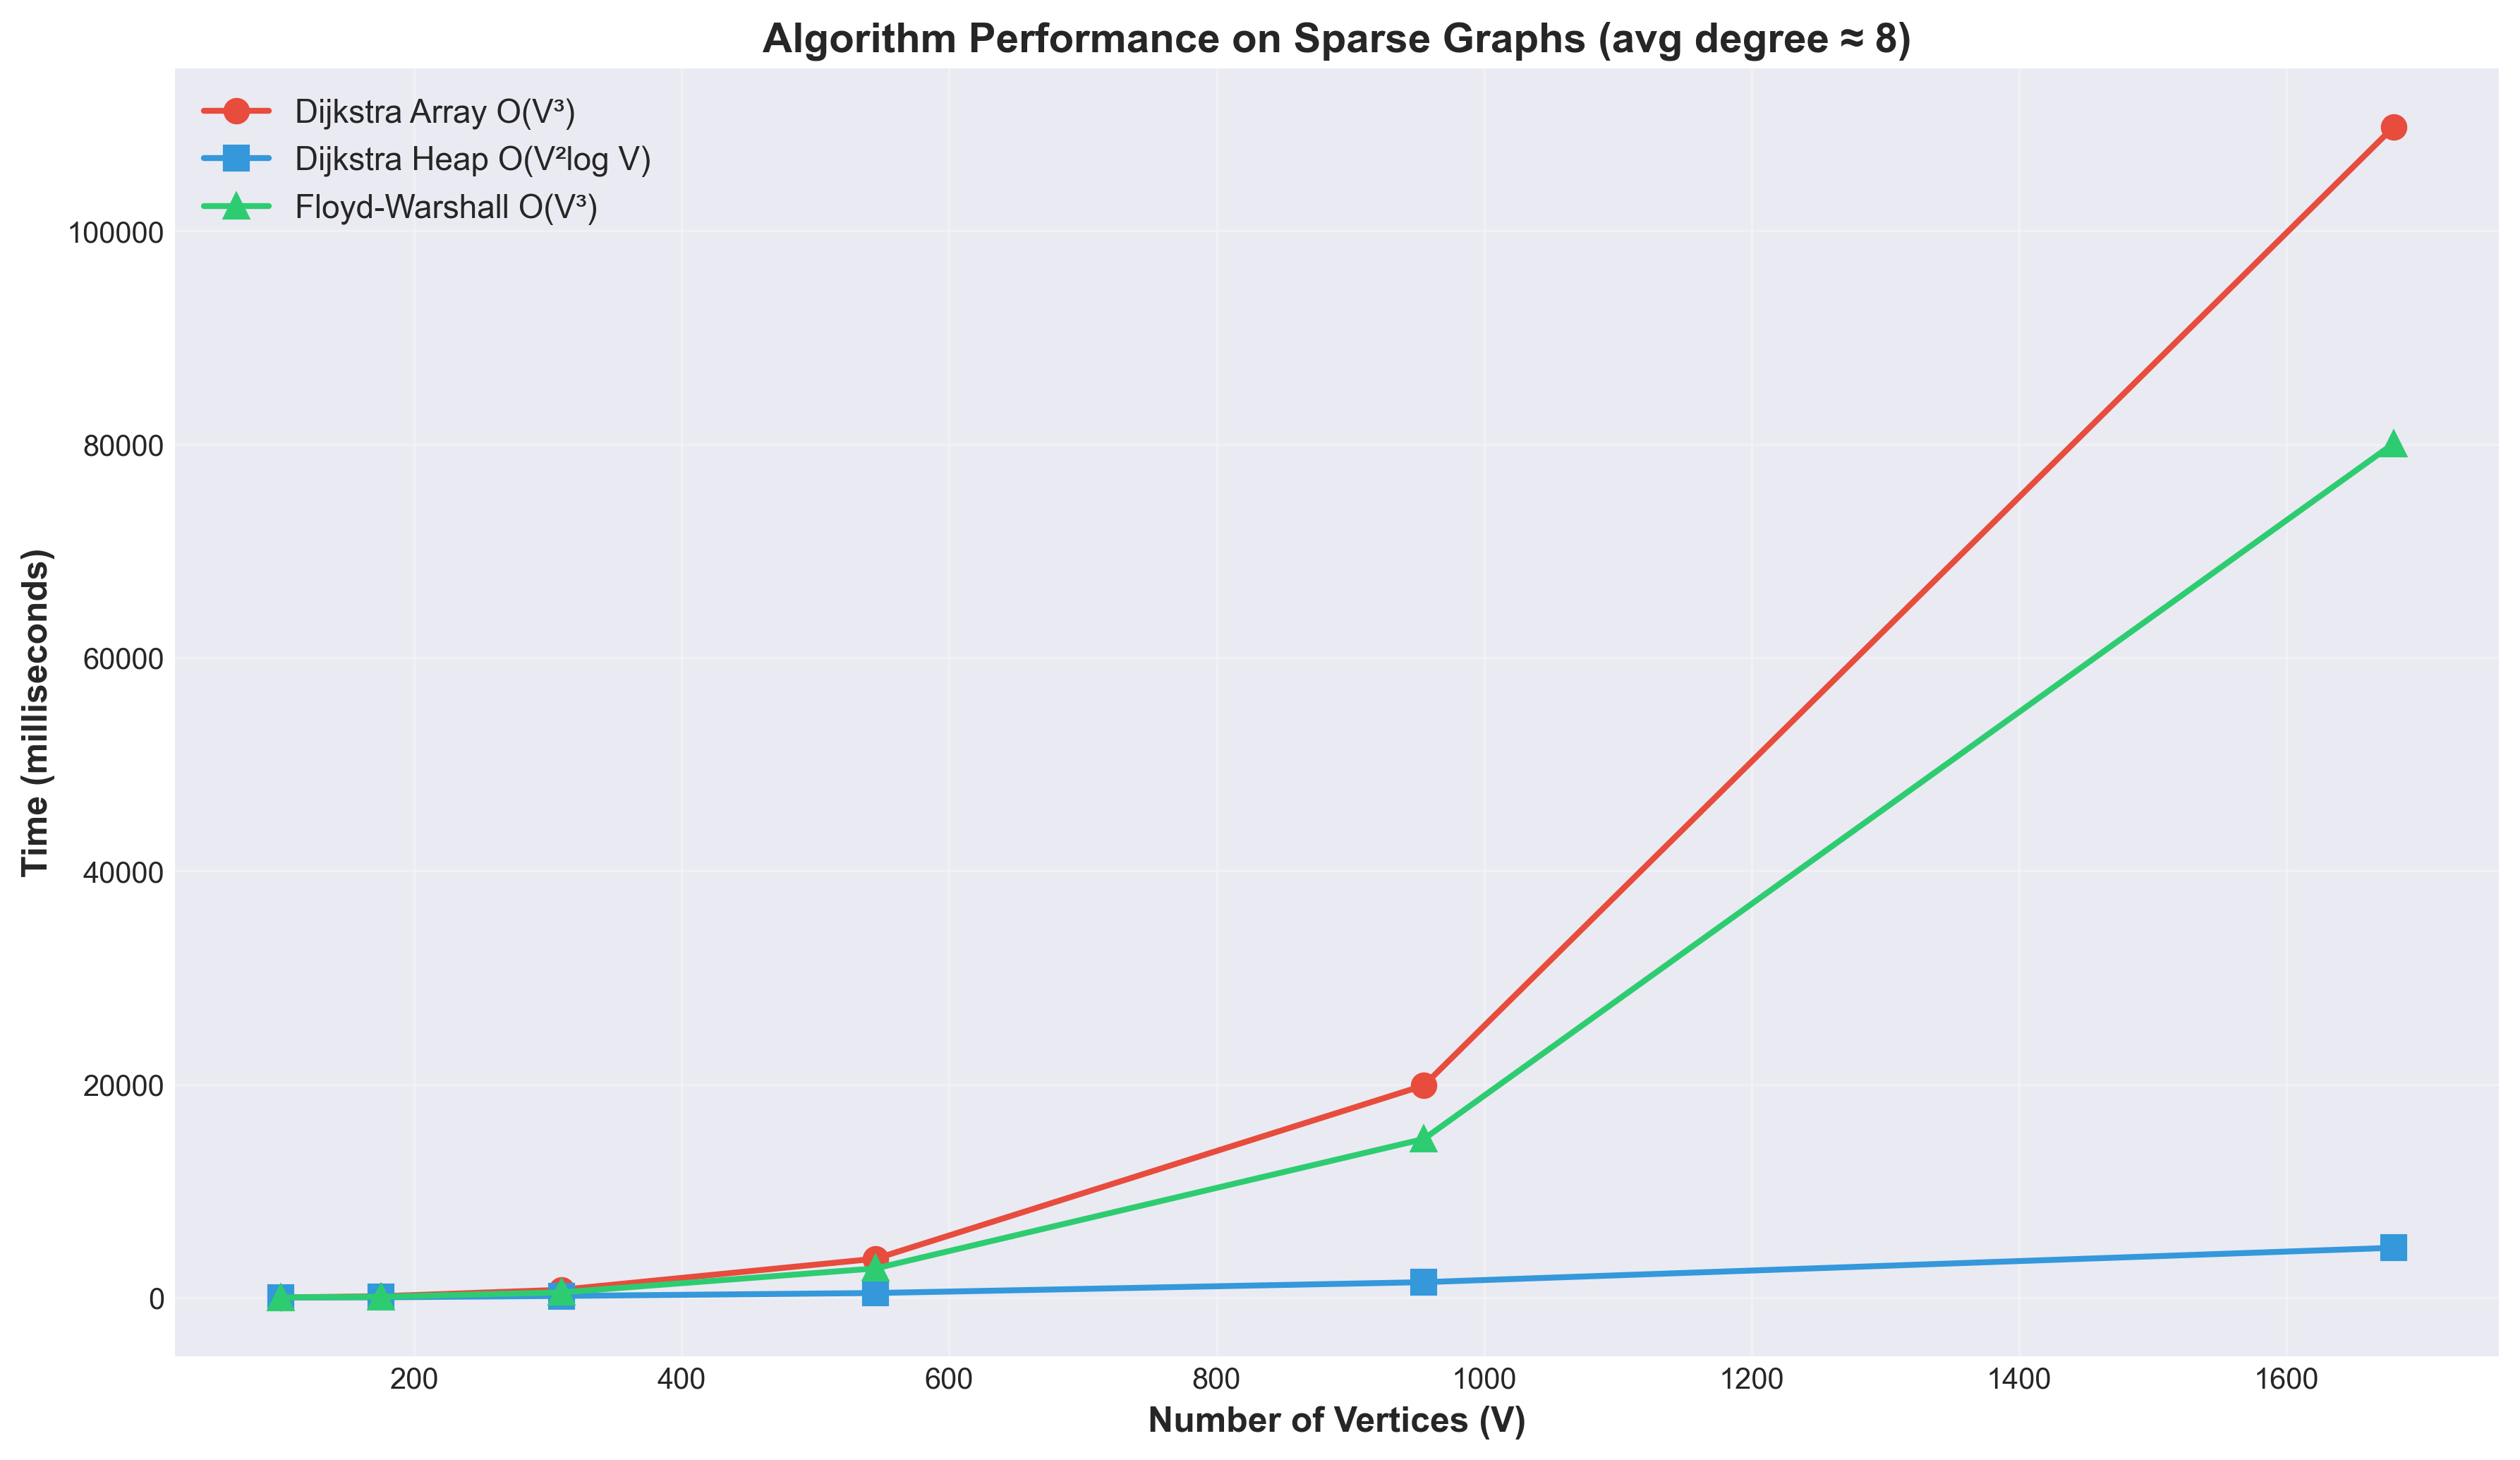
\includegraphics[width=0.95\linewidth]{sparse_comparison.png}
  \caption{Algorithm performance on sparse graphs (average degree $\approx$ 8)}
  \label{fig:sparse}
\end{figure}

\textbf{Key observations:}

\begin{dashenum}
  \item \textbf{Heap-based Dijkstra dominates:} At $V = 1680$, heap-based Dijkstra completed in 4.68 seconds, compared to 109.73 seconds for array-based Dijkstra and 80.06 seconds for Floyd-Warshall. This represents a \textbf{23.4$\times$ speedup} over the array implementation.
  
  \item \textbf{Floyd-Warshall outperforms array-based Dijkstra:} Despite both having $O(V^3)$ complexity, Floyd-Warshall runs approximately 1.4$\times$ faster. This is likely due to better cache locality — the triple nested loop accesses memory in a predictable pattern, while Dijkstra's graph traversal exhibits more irregular memory access.
  
  \item \textbf{Scaling behavior matches theory:} Heap-based Dijkstra shows approximately $O(V^2 \log V)$ scaling, while both array-based Dijkstra and Floyd-Warshall exhibit clear cubic growth.
  
  \item \textbf{Crossover point:} For very small graphs ($V < 175$), the overhead of heap operations makes array-based Dijkstra competitive. However, this advantage quickly disappears as graph size increases.
\end{dashenum}

The average speedup of heap-based Dijkstra over array-based across all sparse graphs is \textbf{9.2$\times$}, confirming the theoretical superiority of the heap approach for sparse graphs.

\section{Performance on Dense Graphs}

Figure~\ref{fig:dense} shows results for dense graphs with 25\% edge density. The performance characteristics shift notably:

\begin{figure}[ht]
  \centering
  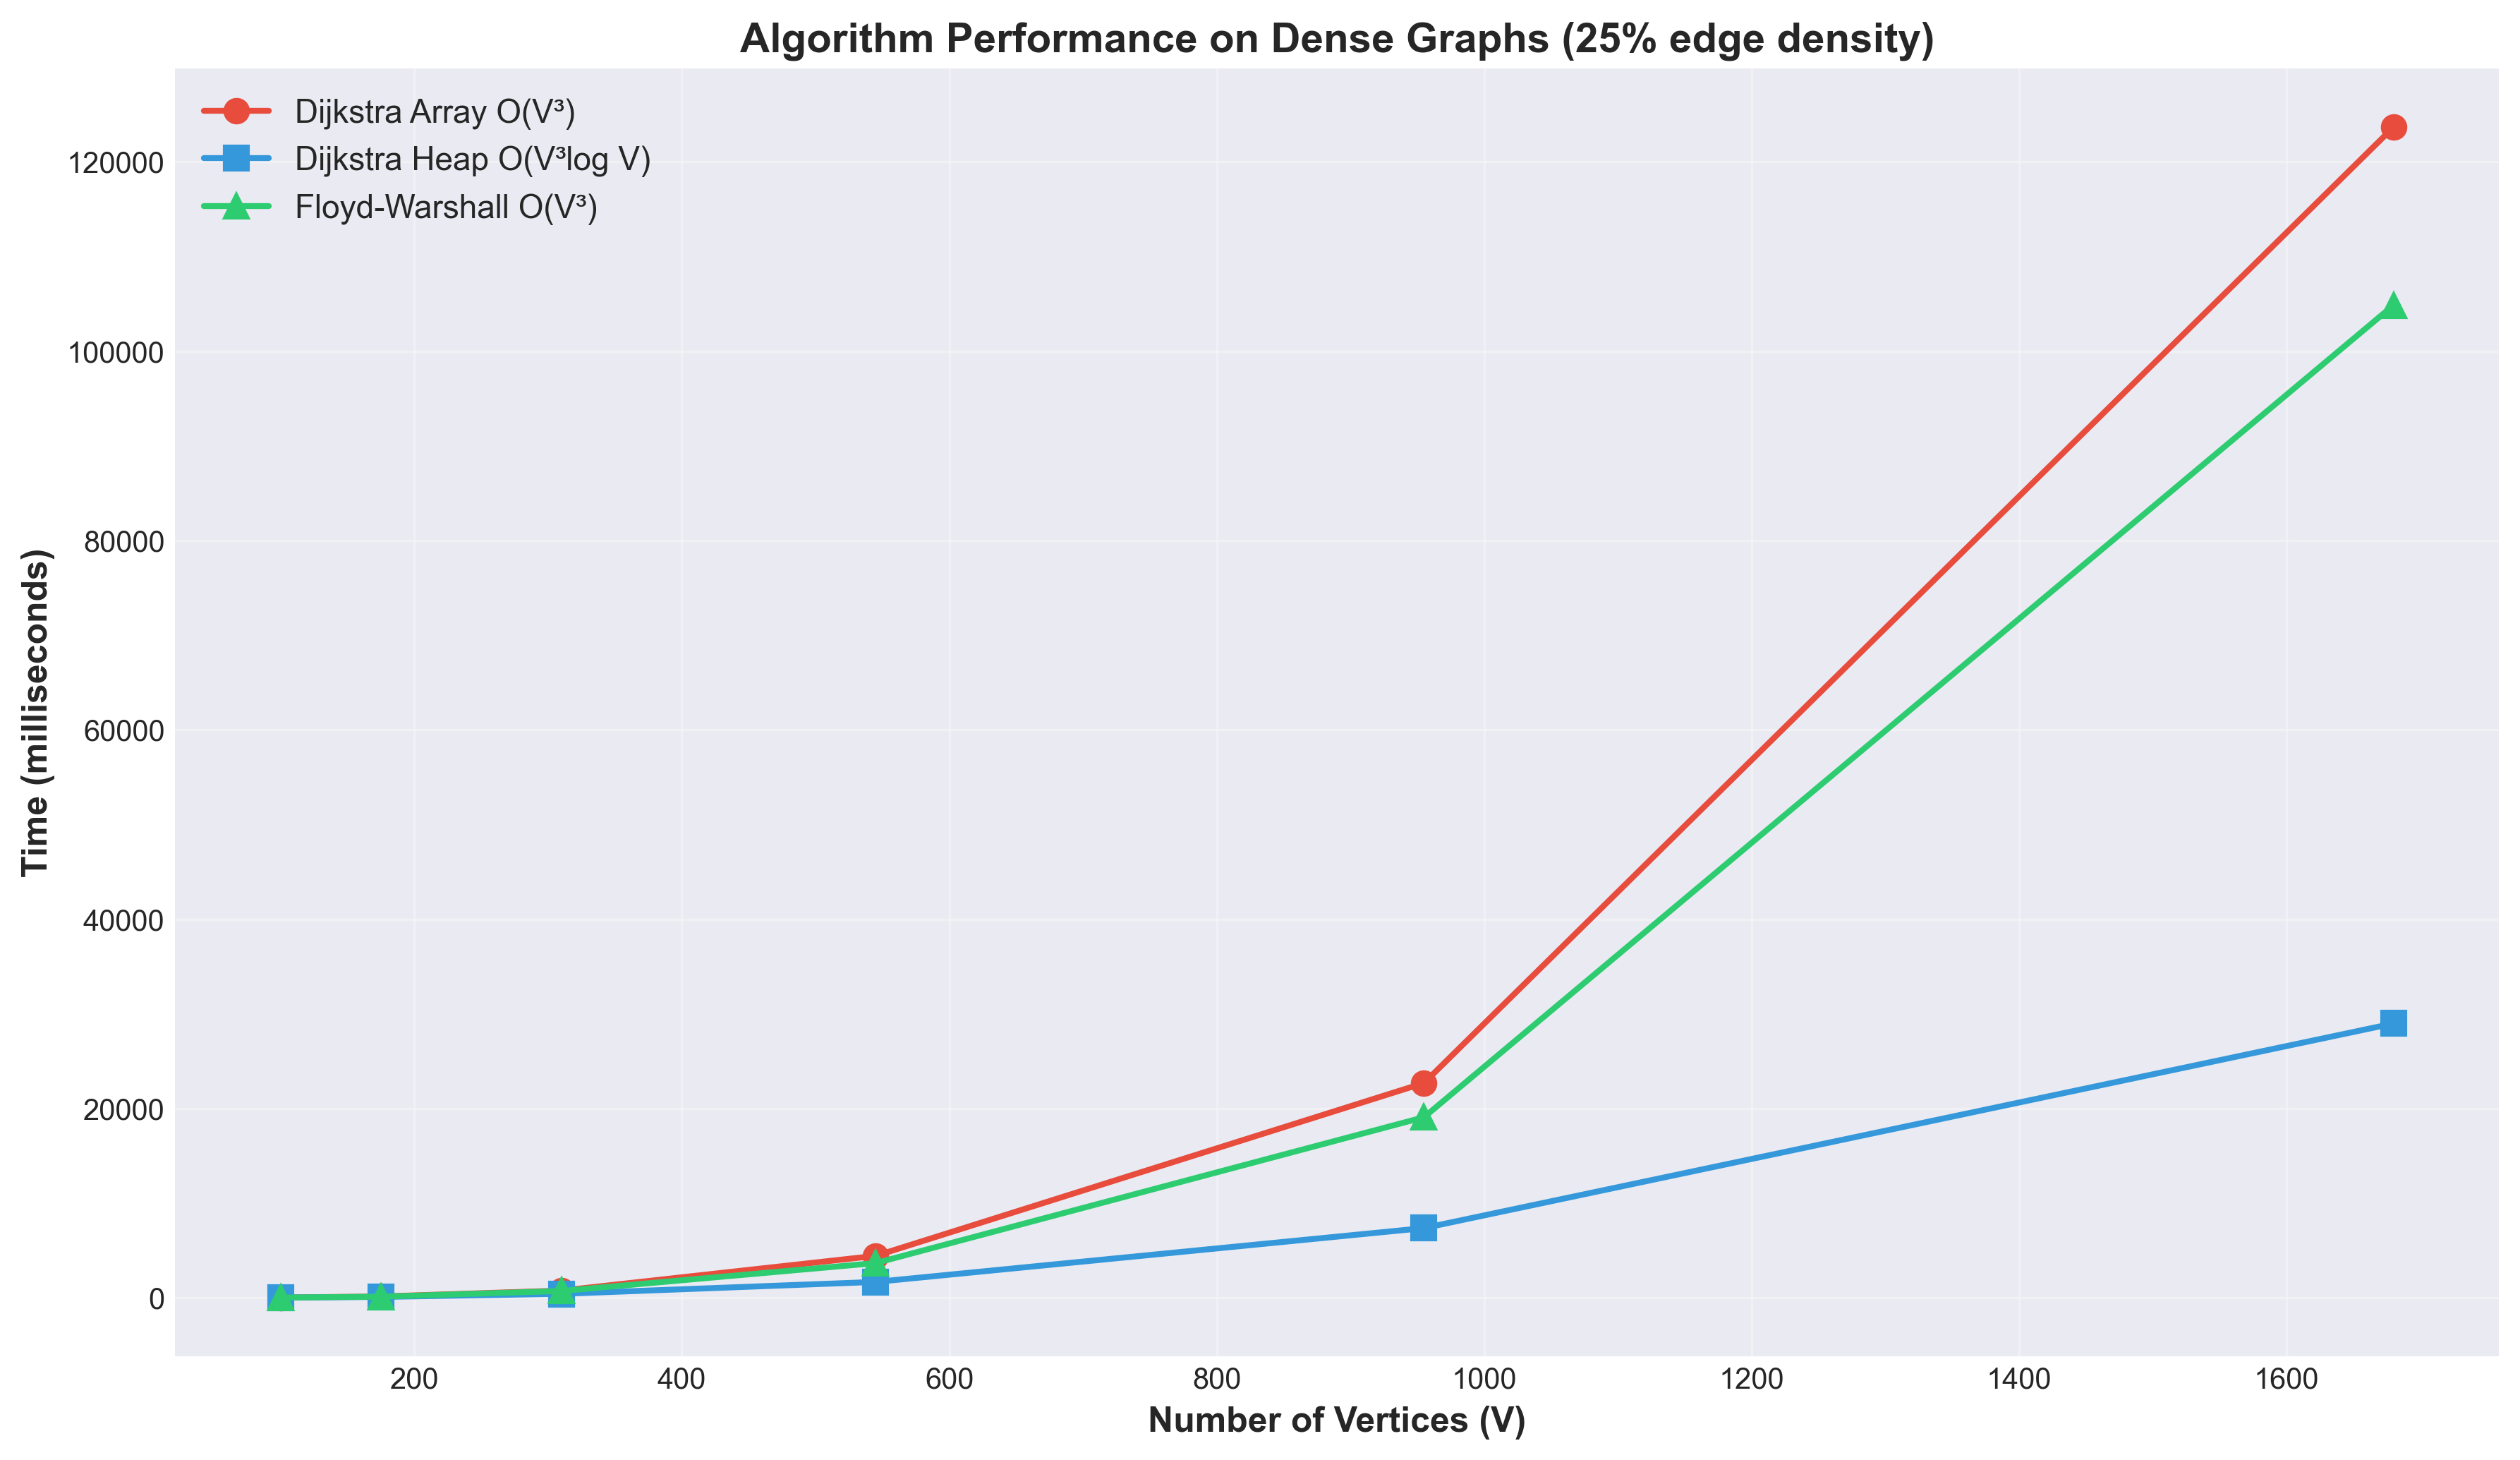
\includegraphics[width=0.95\linewidth]{dense_comparison.png}
  \caption{Algorithm performance on dense graphs (25\% edge density)}
  \label{fig:dense}
\end{figure}

\textbf{Key observations:}

\begin{dashenum}
  \item \textbf{Floyd-Warshall becomes competitive:} At $V = 1680$, Floyd-Warshall (104.85 seconds) slightly outperforms array-based Dijkstra (123.66 seconds), demonstrating the efficiency of its simple triple loop for dense graphs.
  
  \item \textbf{Heap advantage diminishes but persists:} Heap-based Dijkstra still achieves a \textbf{4.3$\times$ speedup} at the largest graph size, though this is significantly less than the 23.4$\times$ speedup observed on sparse graphs. The average speedup across all dense graphs is \textbf{2.4$\times$}.
  
  \item \textbf{All algorithms slow down:} Dense graphs contain approximately 30$\times$ more edges than sparse graphs at the same vertex count. This dramatically increases the work performed by all algorithms, particularly Dijkstra variants which must process every edge.
  
  \item \textbf{Convergence of complexities:} For dense graphs where $E \approx V^2$, the heap-based Dijkstra complexity $O(V \cdot (V + E) \log V) = O(V^3 \log V)$ becomes less favorable compared to the pure $O(V^3)$ of Floyd-Warshall and array-based Dijkstra.
\end{dashenum}

\section{Log-Log Analysis}

Figure~\ref{fig:loglog} presents the same data on logarithmic scales, which linearizes polynomial growth and makes algorithmic complexity visible as slope:

\begin{figure}[ht]
  \centering
  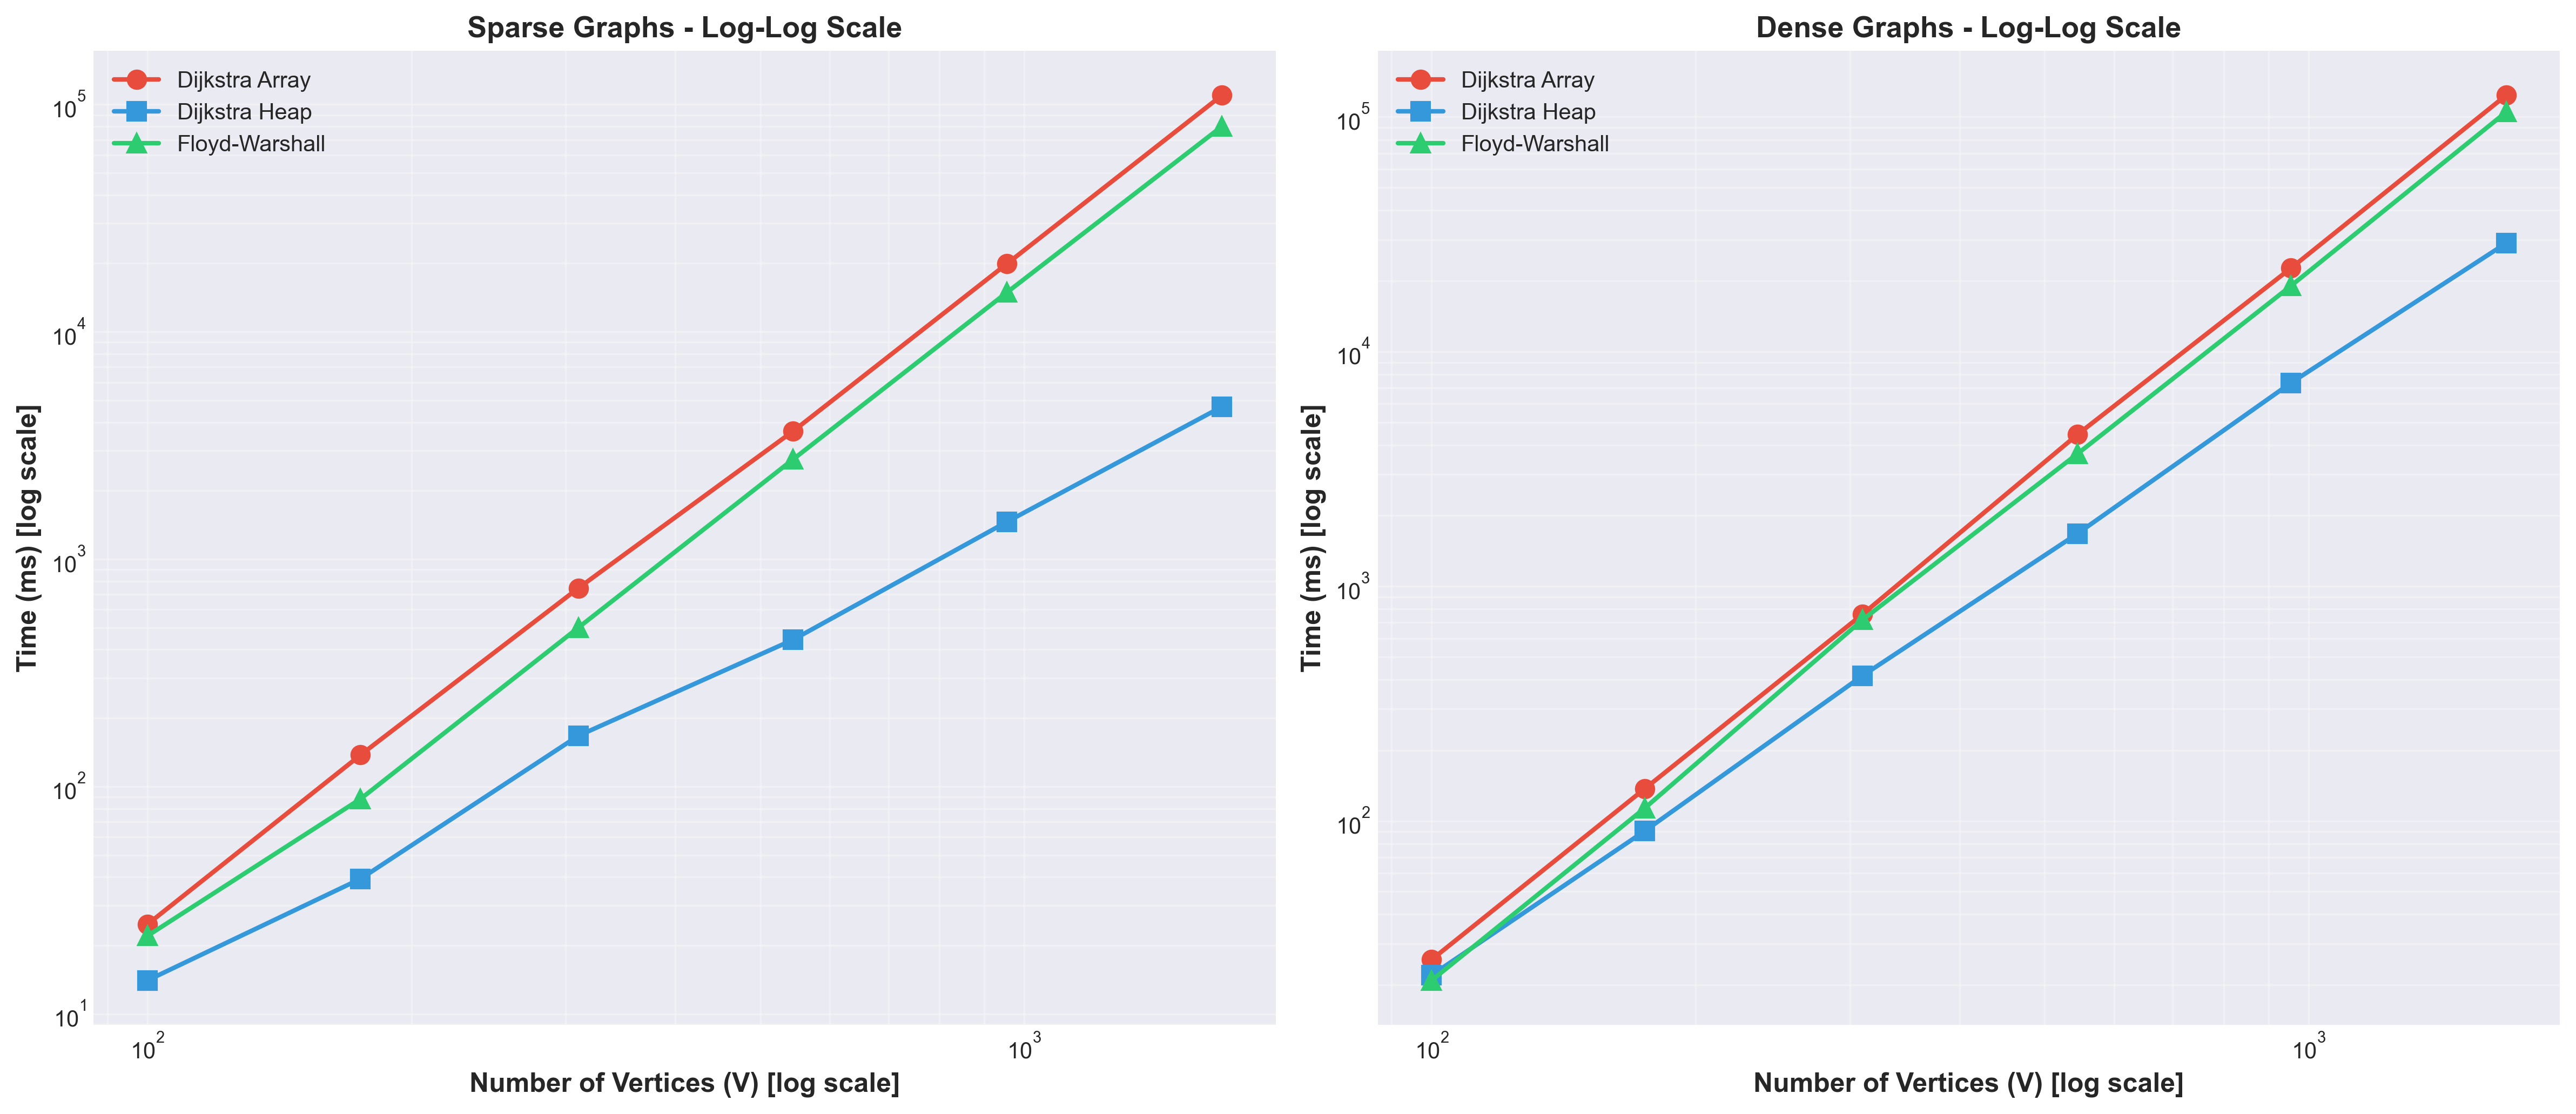
\includegraphics[width=0.95\linewidth]{loglog_comparison.png}
  \caption{Log-log scale comparison showing algorithmic complexity trends}
  \label{fig:loglog}
\end{figure}

On a log-log plot, an algorithm with complexity $O(V^k)$ appears as a straight line with slope $k$. The visualization confirms:

\begin{dashenum}
  \item \textbf{Sparse graphs:} Heap-based Dijkstra shows a slope slightly steeper than 2 (consistent with $O(V^2 \log V)$), while array-based Dijkstra and Floyd-Warshall both exhibit slope 3 (cubic growth).
  
  \item \textbf{Dense graphs:} All three algorithms show slopes approaching 3, with heap-based Dijkstra having a slightly steeper slope due to the additional $\log V$ factor.
  
  \item \textbf{Consistency:} The linearity of all plots confirms that the algorithms behave according to their theoretical complexities across the tested range.
\end{dashenum}

\section{Speedup Analysis}

Figure~\ref{fig:speedup} quantifies the performance advantage of heap-based over array-based Dijkstra as a function of graph size:

\begin{figure}[ht]
  \centering
  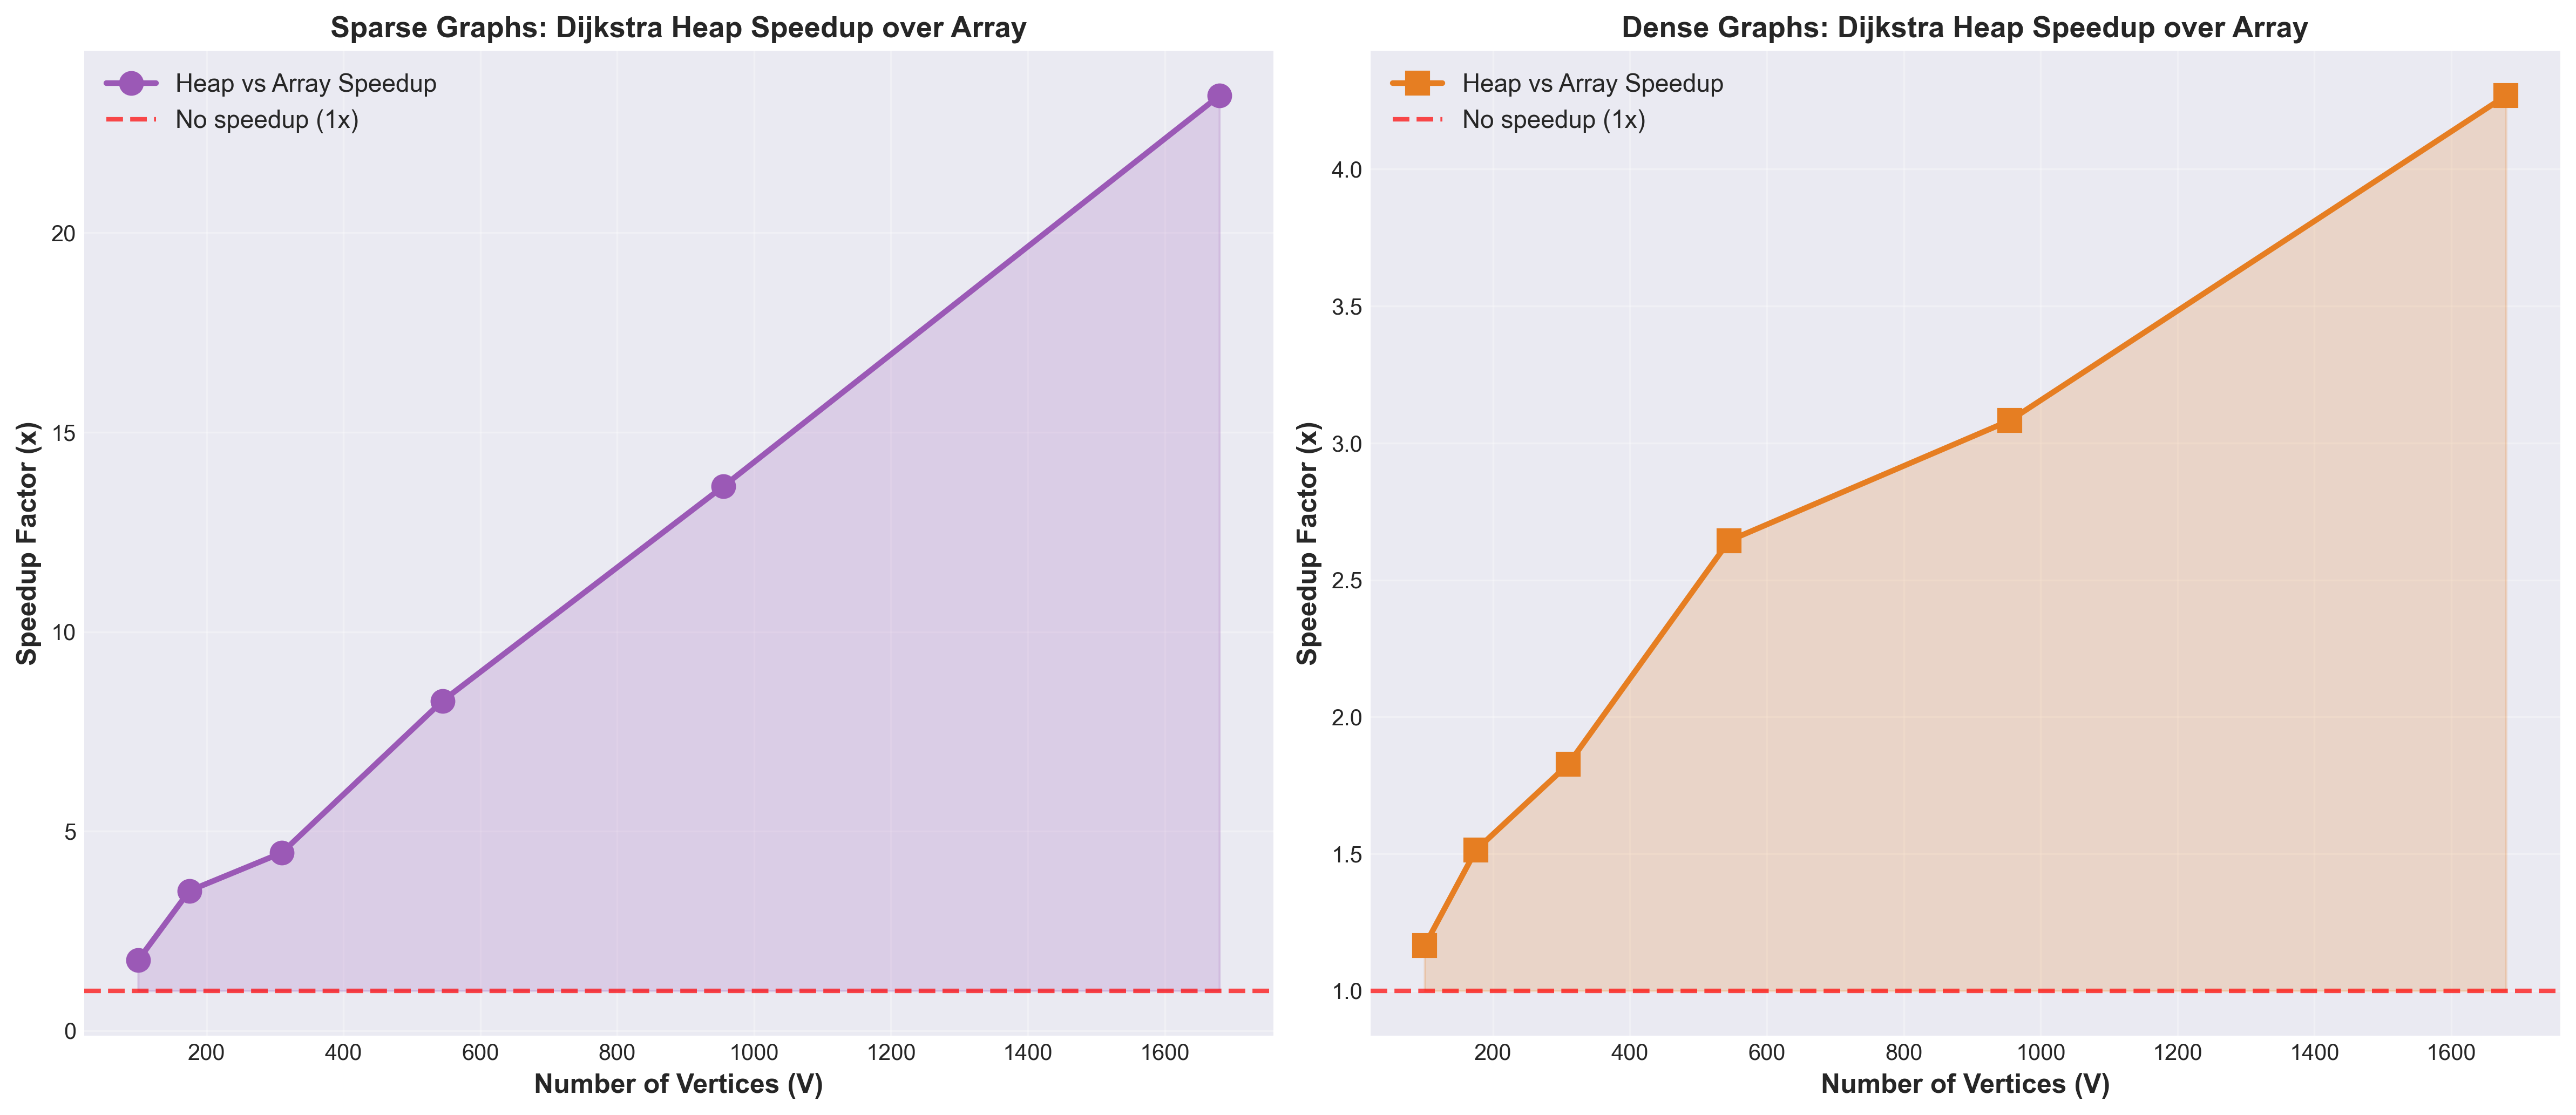
\includegraphics[width=0.95\linewidth]{speedup_analysis.png}
  \caption{Speedup factor: heap-based Dijkstra relative to array-based}
  \label{fig:speedup}
\end{figure}

\textbf{Sparse graph speedup:} The speedup grows from 1.8$\times$ at $V = 100$ to 23.4$\times$ at $V = 1680$, demonstrating that the heap advantage increases with graph size. This matches the theoretical prediction: the $\log V$ factor in the heap complexity becomes increasingly significant as $V$ grows, while the constant-factor overhead of heap operations becomes proportionally less important.

\textbf{Dense graph speedup:} The speedup is more modest, ranging from 1.2$\times$ to 4.3$\times$. Interestingly, the speedup reaches a local maximum around $V = 545$ before slightly declining. This is likely due to cache effects — at very large sizes, the dense graph's adjacency matrix no longer fits in cache, degrading performance for both implementations but affecting the heap variant more due to its less predictable memory access pattern.

\textbf{Practical implications:} For sparse graphs, heap-based Dijkstra is the clear winner and should always be preferred. For dense graphs, the choice is less obvious — Floyd-Warshall's simplicity and slight performance advantage may make it preferable despite Dijkstra's theoretical superiority.

\section{Combined Overview}

Figure~\ref{fig:combined} presents all six algorithm-density combinations on a single plot:

\begin{figure}[ht]
  \centering
  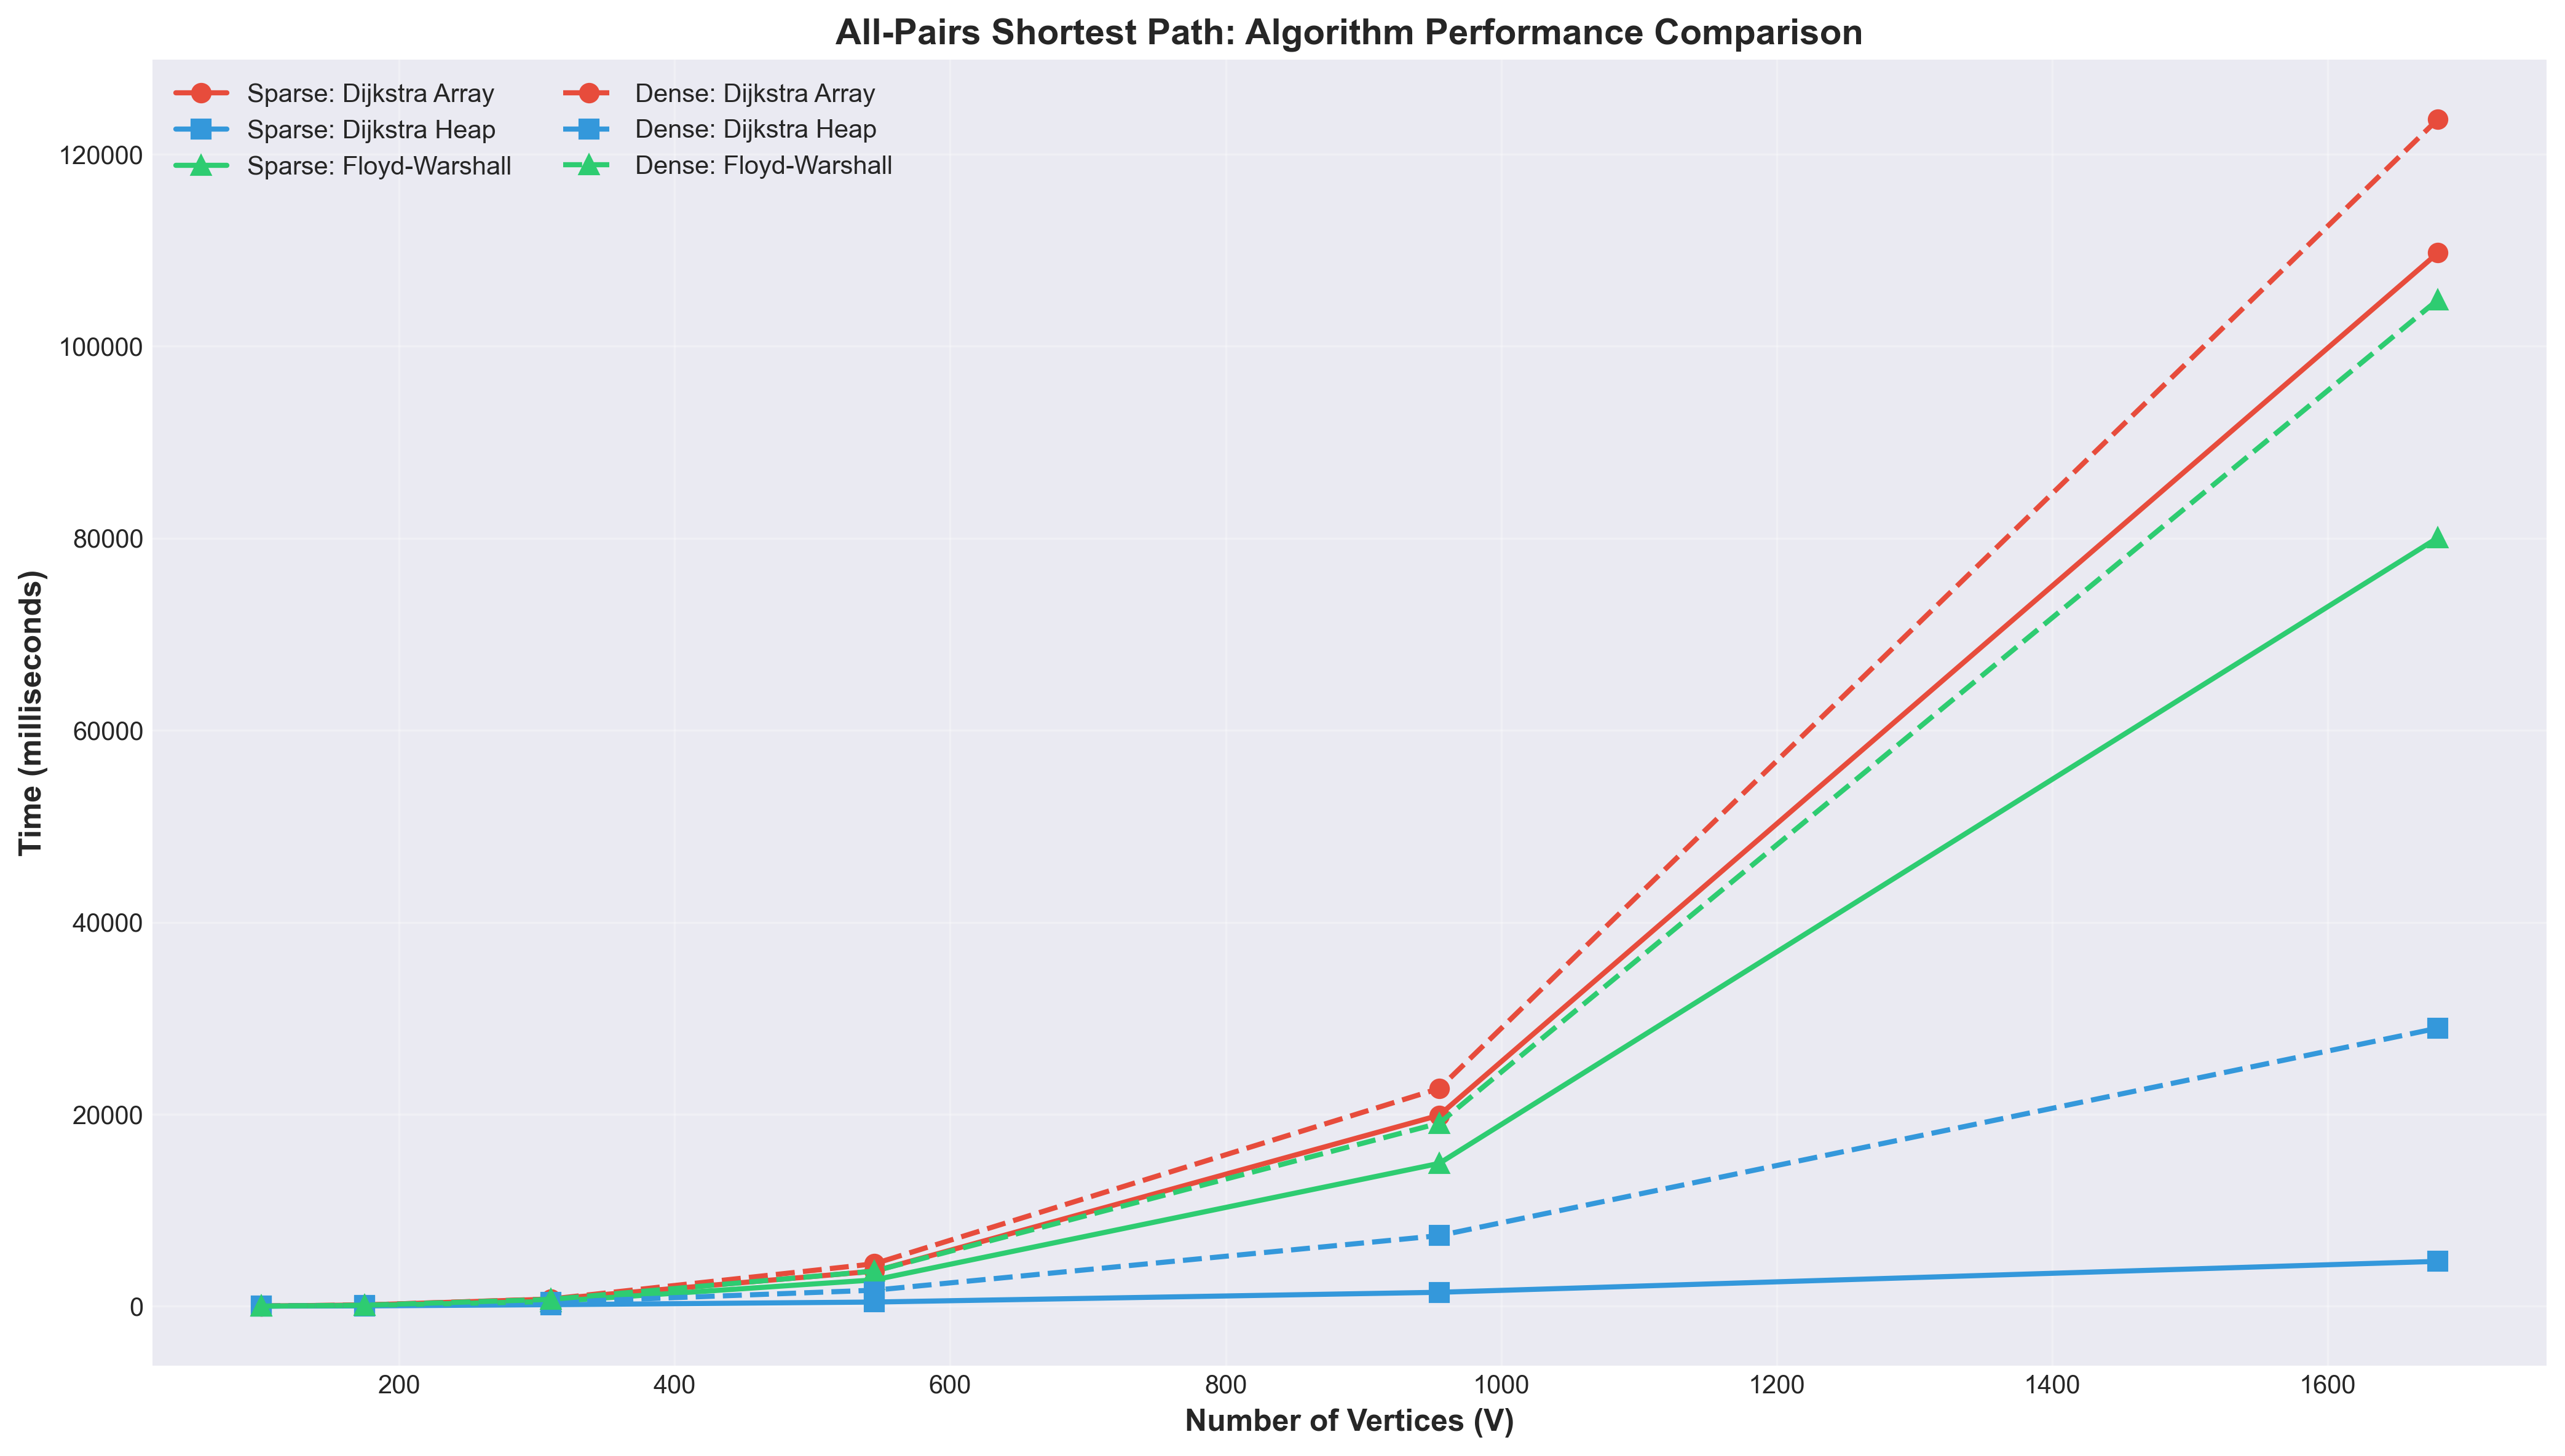
\includegraphics[width=0.95\linewidth]{combined_overview.png}
  \caption{Comprehensive comparison: all algorithms on both sparse and dense graphs}
  \label{fig:combined}
\end{figure}

This visualization emphasizes several key points:

\begin{dashenum}
  \item \textbf{Graph density matters more than algorithm choice for large graphs:} At $V = 1680$, the fastest algorithm on dense graphs (heap-based Dijkstra at 28.97 seconds) is still 6.2$\times$ slower than the same algorithm on sparse graphs (4.68 seconds).
  
  \item \textbf{Algorithm choice matters most on sparse graphs:} The performance spread between algorithms is much larger on sparse graphs (23.4$\times$ from best to worst) than on dense graphs (4.3$\times$ from best to worst).
  
  \item \textbf{Heap-based Dijkstra is the universal winner:} It achieves the best performance on both sparse and dense graphs across all tested sizes, though the margin of victory varies.
  
  \item \textbf{Floyd-Warshall is remarkably stable:} Its performance is nearly identical on sparse and dense graphs when normalized by vertex count, since it depends only on $V$ and not on $E$.
\end{dashenum}

\section{Summary of Findings}

Table~\ref{tab:summary} summarizes the execution times for the largest tested graph ($V = 1680$):

\begin{table}[ht]
\centering
\caption{Execution time comparison at $V = 1680$ vertices}
\label{tab:summary}
\begin{tabular}{lccc}
\toprule
\textbf{Algorithm} & \textbf{Sparse (s)} & \textbf{Dense (s)} & \textbf{Speedup} \\
\midrule
Dijkstra Array     & 109.73              & 123.66             & 1.0$\times$ \\
Dijkstra Heap      & 4.68                & 28.97              & \textbf{23.4$\times$ / 4.3$\times$} \\
Floyd-Warshall     & 80.06               & 104.85             & 1.4$\times$ / 0.8$\times$ \\
\bottomrule
\end{tabular}
\end{table}

\textbf{Recommendations:}
\begin{dashenum}
  \item \textbf{For sparse graphs ($E \ll V^2$):} Use heap-based Dijkstra (all-pairs) or a single-source Dijkstra call for point-to-point queries.
  \item \textbf{For dense graphs ($E \approx V^2$):} Floyd-Warshall is simpler to implement and performs comparably; heap-based Dijkstra is faster but more complex.
  \item \textbf{For graphs with negative edges:} Only Floyd-Warshall or Bellman-Ford can be used; Dijkstra fails.
  \item \textbf{For very large graphs:} Consider specialized algorithms like bidirectional search, A*, or contraction hierarchies.
\end{dashenum}

% ============================================================
%  CHAPTER 4 — CONCLUSION
% ============================================================
\chapter{CONCLUSION}

This laboratory work provided empirical validation of the theoretical complexity analysis for three approaches to solving the all-pairs shortest path problem: array-based Dijkstra, heap-based Dijkstra, and Floyd-Warshall.

\textbf{Key findings:}

\begin{dashenum}
  \item \textbf{Heap-based Dijkstra is the clear winner for sparse graphs.} The 23.4$\times$ speedup at $V = 1680$ demonstrates the dramatic practical advantage of using an efficient priority queue implementation. This speedup grows with graph size, making the heap approach essential for large sparse graphs.
  
  \item \textbf{Floyd-Warshall remains competitive for dense graphs.} Its simple triple loop achieves excellent cache locality and performs comparably to array-based Dijkstra despite identical asymptotic complexity. For dense graphs, its simplicity may outweigh the modest performance advantage of heap-based Dijkstra.
  
  \item \textbf{Graph representation matters.} The choice between adjacency list (for Dijkstra) and adjacency matrix (for Floyd-Warshall) has significant performance implications. Adjacency lists excel for sparse graphs, while matrices are mandatory for Floyd-Warshall and competitive for dense graphs.
  
  \item \textbf{Theory and practice align.} The empirical results closely match theoretical complexity predictions. Heap-based Dijkstra exhibits $O(V^2 \log V)$ scaling on sparse graphs, while all $O(V^3)$ algorithms show clear cubic growth.
  
  \item \textbf{Implementation details matter.} The overhead of heap operations makes array-based Dijkstra competitive for very small graphs ($V < 175$), but this advantage disappears rapidly as size increases.
\end{dashenum}

\textbf{Practical implications:}

The choice of algorithm should be guided by graph characteristics:
\begin{dashenum}
  \item Sparse graphs with $E = O(V)$ or $E = O(V \log V)$ strongly favor heap-based Dijkstra
  \item Dense graphs with $E = \Theta(V^2)$ make Floyd-Warshall a reasonable choice
  \item The presence of negative edge weights eliminates Dijkstra as an option
  \item For single-source queries, even a single Dijkstra call often suffices
\end{dashenum}

\textbf{Dynamic programming perspective:}

Both algorithms exemplify dynamic programming principles:
\begin{dashenum}
  \item \textbf{Dijkstra:} Maintains optimal substructure through the distance array, using greedy selection combined with relaxation to build optimal paths incrementally
  \item \textbf{Floyd-Warshall:} Explicitly constructs a recurrence relation over intermediate vertices, solving subproblems in a well-defined order
\end{dashenum}

This laboratory successfully demonstrated how theoretical algorithm analysis translates to practical performance, providing concrete evidence for algorithm selection in real-world applications. The empirical approach validated asymptotic complexity predictions while revealing important constant-factor differences and implementation considerations that theory alone cannot capture.

% ============================================================
%  REFERENCES
% ============================================================
\begin{thebibliography}{99}
\addcontentsline{toc}{chapter}{References}
\markboth{References}{References}
\thispagestyle{plain}

\bibitem{ref:dp}
  GeeksforGeeks. \textit{Dynamic Programming}.
  Available at: \url{https://www.geeksforgeeks.org/dynamic-programming/}
  [accessed: April 28, 2026].

\bibitem{ref:dijkstra}
  GeeksforGeeks. \textit{Dijkstra's Shortest Path Algorithm}.
  Available at: \url{https://www.geeksforgeeks.org/dijkstras-shortest-path-algorithm-greedy-algo-7/}
  [accessed: April 28, 2026].

\bibitem{ref:floyd}
  GeeksforGeeks. \textit{Floyd Warshall Algorithm}.
  Available at: \url{https://www.geeksforgeeks.org/floyd-warshall-algorithm-dp-16/}
  [accessed: April 28, 2026].

\bibitem{ref:cormen}
  Cormen, T. H., Leiserson, C. E., Rivest, R. L., and Stein, C. (2009).
  \textit{Introduction to Algorithms}, 3rd edition.
  MIT Press, Cambridge, MA.

\bibitem{ref:comparison}
  Coding Ninjas. \textit{Dijkstra's Algorithm vs Floyd-Warshall's Algorithm}.
  Available at: \url{https://www.codingninjas.com/codestudio/library/dijkstras-algorithm-vs-floydwarshalls-algorithm}
  [accessed: April 28, 2026].

\bibitem{ref:github}
  Bruma, C. (2026). \textit{Dijkstra and Floyd-Warshall: Implementation and Empirical Analysis}.
  GitHub repository. 
  Available at: \url{https://github.com/Makday/UTM_AA_course_2025-2026}
  [accessed: April 28, 2026].

\end{thebibliography}

\end{document}